\documentclass[11pt]{article}
\usepackage[T1]{fontenc}
\usepackage{lmodern,microtype}
\usepackage[margin=1in]{geometry}
\usepackage{amsmath,amssymb,amsthm,mathtools,booktabs,array,longtable,graphicx,xcolor}
\usepackage[colorlinks=true,linkcolor=blue!45!black,citecolor=blue!45!black,urlcolor=blue!45!black]{hyperref}
\usepackage[nameinlink,noabbrev]{cleveref}
\hypersetup{pdftitle={Partial-Population Inference on Classical Data},pdfauthor={Christopher D. Long},pdfsubject={Certified projection, calibration choices, and classical observations}}
\setlength{\emergencystretch}{3em}
\makeatletter\newcommand{\tableinput}[1]{\@@input #1 }\makeatother
\newtheorem{theorem}{Theorem}[section]
\newtheorem{proposition}[theorem]{Proposition}
\theoremstyle{remark}\newtheorem{remark}[theorem]{Remark}
\newcommand{\E}{\mathbb E}\newcommand{\PP}{\mathbb P}
\newcommand{\dd}{\,\mathrm d}\newcommand{\ind}{\mathbf1}
\title{Partial-Population Inference on Classical Data:\\Discovery, Recapture, and Serial Numbers}
\author{Christopher D. Long}
\date{November 17, 2026\\Research draft, version 0.1}
\begin{document}\maketitle
\begin{abstract}
We implement certified outer projections of a fixed-design joint confidence
region for realized missing mass and realized future discoveries. A finite-grid
conic optimizer proposes dual weights; interval arithmetic verifies the
population kernels over the entire probability domain, and an entropy
inequality certifies the projected endpoints. Feasible relaxed measures provide
separate bounds on optimization error. We apply the construction to Corbet
butterflies, Rothamsted moths, Preston birds, Shakespeare word frequencies, and
Barro Colorado Island tree counts, and report capture--recapture estimates for
Dahl trout, snowshoe hares, Edwards--Eberhardt cottontails, and fifteen textbook
frequency series, including Carothers taxis. Truncated tables, sampling-design
limitations, and conflicting source summaries are preserved explicitly. A
known-removal extension handles Gerking's sunfish experiment. A paired
simulation compares coverage and width on four specified populations
at two sample sizes. The certified intervals are conservative and only modestly
narrower than a separately calibrated construction using the same directions;
normal Good--Turing calibrations are much narrower and are reproduced as
explicit choices within the framework, with their approximation assumptions.
Every continuum certificate and simulated target is saved for replay.
The historical serial-number section documents an archival source but does not
substitute invented data for an unrecovered wartime sample. This is a reproducible
computational extension of the companion theory, not a claim of new classical
estimators, shortest intervals, or empirical validation of an iid model for
historical observational data.
\end{abstract}

\section{Experiments, targets, and the scope of the comparison}
Let $p=(p_i)$ be a probability distribution on a finite or countable set of
species or word types. An initial iid sample of fixed size $n$ has counts $X_i$
and fingerprint $\Phi_r=\sum_i\ind\{X_i=r\}$. Its realized missing mass is
\[
 M=\sum_i p_i\ind\{X_i=0\}.
\]
Given an independent future iid sample of a prespecified size $m$, with counts
$X'_i$, the realized number of discoveries is
\[
 Y_m=\sum_i\ind\{X_i=0,\ X'_i>0\}.
\]
These are different random targets. In particular, an interval for $Y_m$ is
a prediction interval and is not automatically an interval for
$\E[Y_m\mid X]$, $\E Y_m$, total richness, or the vocabulary a writer knew.
Our guarantees are unconditional over the indicated samples. They are not
conditional on the observed fingerprint. All reported nominal levels are 95\%.

The companion papers develop the recovery identities, transfer principles,
and calibration machinery \cite{LongDiscovery,LongTransfer,LongCumulants,LongCapture}.
Here we implement one specified region: eight directions, equal mixture
weights, fixed Poisson efforts $t=n$ and $u=m$, and the whole relaxed
probability-measure class. We do not optimize effort, combine full deletion
scores, enforce integer realizability, or claim a uniformly shortest interval.
Those distinctions matter because stronger theory alone does not establish
that a particular numerical routine computes its sharpest consequence.

Capture--recapture uses a different experiment. Two uniform samples of sizes
$a,b$ from a closed population of size $N$ have overlap
$J\sim\operatorname{Hypergeom}(N,a,b)$. Repeated histories require their
occasion order for the Schnabel and Schumacher--Eschmeyer ratios. Frequency
tables alone support different summaries. Serial-number magnitudes carry
information in the German tank experiment that arbitrary capture labels do
not. We retain these distinctions throughout.

\section{The joint region computed here}
\subsection{Poisson factors and fixed-count calibration}
Write $\nu_p=\sum_i p_i\delta_{p_i}$, a probability measure on $(0,1]$.
For one direction $(\lambda,\eta)$, where $\lambda=(\lambda_1,\ldots,\lambda_d)$,
define, for $x>0$,
\begin{align}
 f_M(x)&=1+e^{-nx}\sum_{r=1}^d\frac{(nx)^r}{r!}(e^{\lambda_r}-1)
                  +e^{-nx}(e^{\eta x}-1),\label{eq:factorM}\\
 f_Y(x)&=1+e^{-nx}\sum_{r=1}^d\frac{(nx)^r}{r!}(e^{\lambda_r}-1)
                  +e^{-nx}(1-e^{-mx})(e^\eta-1),\label{eq:factorY}\\
 \kappa(x)&=x^{-1}\log f(x).
\end{align}
These are positive moment-generating factors under independent Poisson
counts. Their continuous extensions at zero are
\[
 \kappa_M(0)=n(e^{\lambda_1}-1)+\eta,\qquad
 \kappa_Y(0)=n(e^{\lambda_1}-1)+m(e^\eta-1).
\]
Set $h_n=-\log\PP\{\operatorname{Pois}(n)=n\}$ and let $h=h_n$ for mass,
$h=h_n+h_m$ for discoveries. If $T=M$ or $T=Y_m$, respectively, then
\begin{equation}\label{eq:evalue}
 E_{\lambda,\eta}(\nu,T)
 =\exp\left\{\lambda\cdot\Phi+\eta T-h-\int\kappa\dd\nu\right\}
\end{equation}
has expectation at most one at $(\nu_p,T)$ under the corresponding fixed-count
experiment. Indeed, before conditioning, the factorization gives expectation
one. Conditional expectation is at most the unconditional expectation divided
by the probability of the conditioning event. Multiplication by $e^{-h}$
compensates for that division. The initial and future total counts are
independent Poisson variables in the prediction construction. Bounded continuous
$\kappa$ and $\nu_p([0,1])=1$ also justify the countable-population transform
as in the companion cumulant paper.

\subsection{Predetermined directions}
The numerical implementation fixes
\[
 b_n=\left[\max\left\{4,\left\lceil\sqrt{\frac{n}{\log(n+1)+3}}\right\rceil\right\}\right]^{-1},
 \qquad s\in b_n\{-2,-1,-\tfrac12,-\tfrac14,\tfrac14,\tfrac12,1,2\}.
\]
The actual rational scales are serialized with every design, so replay does
not depend on recomputing a floating-point ceiling. For mass, use
$d=1$, $\lambda_1=-s$, $\eta=sn$. For discoveries, use $d=3$,
\[
 \lambda_r=-s(-1)^{r+1}(m/n)^r\quad(1\le r\le3),\qquad \eta=s.
\]
The latter is a three-coordinate Good--Toulmin-type score, not an assertion
that the truncated point predictor is unbiased. Arbitrary fixed coefficients
are calibrated by \eqref{eq:factorY}; truncation affects efficiency, not this
validity argument. We examine $m\le n$ in the reported examples. Directions,
weights, sample sizes, and horizons are selected before inspecting their
fingerprints. Optimizing a dual certificate after observing the data does
not change this preassigned region.

For $J=8$, take $F(\nu,T)=J^{-1}\sum_{j=1}^J E_j(\nu,T)$ and let
\begin{equation}\label{eq:region}
 \mathcal C_\alpha(\Phi)=
 \{(\nu,z):\nu\in\mathcal P([0,1]),\ 0\le z\le1,
                      \ F(\nu,Lz)\le\alpha^{-1}\},
 \qquad L=\begin{cases}1&\text{for }M,\\m&\text{for }Y_m.\end{cases}
\end{equation}
The class $\mathcal P([0,1])$ includes the true abundance measure and allows
additional relaxed measures, including mass at zero. It does not impose all
observational consistency or integer-population constraints. The region is
convex and compact when nonempty; its projection on $z$ is an interval.
Markov's inequality gives at least $1-\alpha$ coverage by any outer enclosure
of that projection. For discoveries we intersect the enclosure in $Lz$ with
the integers. An empty reported intersection is replaced by full support.
This conservative convention cannot reduce coverage.

\section{Continuum certificates and computable error bounds}
\subsection{Entropy duality}
Let $q=(q_1,\ldots,q_J)$ be a probability vector, with $0\log0=0$, and write
\begin{align*}
 A(q)&=L\sum_jq_j\eta_j,\\
 B(q)&=\sum_jq_j\{\lambda_j\cdot\Phi-h-\log J-\log q_j\},\\
 H(q)&=\sup_{0\le x\le1}\sum_jq_j\kappa_j(x).
\end{align*}
Terms with $q_j=0$ are omitted in $B$.
\begin{proposition}[Certified projected endpoints]\label{prop:dual}
Suppose $\overline H(q)\ge H(q)$ is a certified bound. Every
$(\nu,z)\in\mathcal C_\alpha(\Phi)$ satisfies
\[
 B(q)+A(q)z-\overline H(q)\le\log(1/\alpha).
\]
Consequently, if $A(q)>0$, an upper endpoint is
$\{\log(1/\alpha)-B(q)+\overline H(q)\}/A(q)$; if $A(q)<0$, the same expression
is a lower endpoint. Intersecting these constraints with $[0,1]$ preserves an
outer enclosure of the projection.
\end{proposition}
\begin{proof}
The entropy form of the log-sum-exp inequality gives
\[
 \log F(\nu,Lz)\ge B(q)+A(q)z
              -\int\sum_jq_j\kappa_j(x)\dd\nu(x)
 \ge B(q)+A(q)z-\overline H(q).
\]
Membership in \eqref{eq:region} bounds the left side above by
$\log(1/\alpha)$. Division by a signed $A(q)$ yields the stated inequalities.
\end{proof}

The conic optimizer searches a finite atom grid only to propose $q$. We
rationalize its nonnegative weights to integers summing exactly to $10^{12}$.
Validity then depends on \cref{prop:dual}, not on the solver's status, grid
resolution, reported objective, or dual residual. In particular a solver
failure cannot turn a numerical guess into a certified answer.

\subsection{Interval arithmetic over the whole domain}
The stored kernel table partitions $[0,1]$ into contiguous cells $I_\ell$ and
records binary64 numbers $U_{\ell j}$ satisfying
$\kappa_j(x)\le U_{\ell j}$ for every $x\in I_\ell$. Since $q_j\ge0$,
\[
 \overline H(q)=\max_\ell\sum_jq_j U_{\ell j}
\]
is sufficient. FLINT/Arb ball arithmetic at 128-bit working precision checks
each entire cell, rather than just its endpoints or grid nodes
\cite{Johansson2017,PythonFlint}. Binary64 conversion is rounded outward and
checked against the ball. The final rescaling to $M$ or $Y_m$ is also rounded
outward. Future counts use the ceiling of the lower bound and floor of the
upper bound only after this rescaling.

At the removable singularity, direct division by an interval containing zero
would fail. Instead, with $f(0)=1$,
\[
 \frac{\log f(x)}x=\int_0^1\frac{f'(sx)}{f(sx)}\dd s.
\]
An enclosure of $f'/f$ over the first cell encloses this integral. Other cells
use direct logarithmic interval evaluation. Exponential differences use
\texttt{expm1} expressions to reduce cancellation; cells producing a nonfinite
enclosure are subdivided. Failure to enclose after the subdivision limit
raises an error. It does not produce a nominally certified interval.

\subsection{Feasible witnesses and fallback behavior}
A second certificate consists of a finite relaxed measure with rational
weights summing to one and a proposed value $z_0$. Direct interval evaluation
checks $F(\nu_0,Lz_0)\le\alpha^{-1}$. If a lower outer bound is $\ell$ and a
feasible witness is $z_\ell$, then the exact lower endpoint of the relaxed
region lies in $[\ell,z_\ell]$. The upper endpoint analogously lies between a
feasible $z_u$ and its outer bound $u$. Tables report these witness-to-bound
gaps in target units. They bound error for the chosen relaxed region, not the
difference from an integer-realizable population model. A missing witness
does not invalidate a dual enclosure but leaves that optimization gap unknown.

CVXPY with CLARABEL supplies the proposals \cite{CVXPY,Clarabel}. On numerical
failure, the implementation chooses the strongest certified bound among
individual directions of the required sign. It retains the mixture penalty
$\log J$. Invalid fingerprints are rejected. The replay path checks shared
kernel tables once and then every rational dual vector, signed endpoint,
reported interval, and available primal witness without calling a conic solver.
This is numerical certification with trusted arithmetic and explicit analytic
proofs, not proof-assistant verification.

\section{Calibration is a choice: recovering Good--Turing approximations}
Conservatism is a property of the selected calibration and nuisance class, not
an intrinsic requirement of the recovery framework. Estimation, studentization,
and calibration can be selected separately. In particular, choosing a normal
approximation recovers the classical Good--Turing interval exactly, rather
than treating it as a method that lies outside the framework.

Under independent Poisson counts at known effort $n$, let $Z=\Phi_1-nM$.
The cumulant construction gives the exact identities
\[
 \E Z=0,\qquad
 \operatorname{Var}(Z)=\E\Phi_1+2\E\Phi_2,\qquad
 \operatorname{Cov}(Z,S)=\E\Phi_1,\quad \operatorname{Var}(S)=n,
\]
where $S$ is the total count. Replacing moments by their observed counterparts
and using Gaussian calibration yields the Poisson-variance interval
\[
 \Phi_1/n\ \pm\ z_{1-\alpha/2}\sqrt{(\Phi_1+2\Phi_2)/n^2}.
\]
Gaussian conditioning on $S=n$ suggests the Schur-complement correction
$\operatorname{Var}(Z)-\operatorname{Cov}(Z,S)^2/n$, hence the fixed-count
studentizer $(\Phi_1+2\Phi_2-\Phi_1^2/n)/n^2$. This explains the correction;
an ordinary joint CLT alone is not sufficient to justify conditioning on an
event of vanishing probability. The applicable fixed-count limit theorem,
or a suitable local-limit conditioning argument, supplies that justification
\cite{Esty1983,ZhangZhang2009}.

The approximation requires nondegenerate error variance, a Lindeberg-type
condition preventing a few rare events from dominating the standardized
error, consistent studentization, and negligible standardized bias. At fixed
$n$ the exact bias is
\[
 \E(\Phi_1/n-M)=\sum_i p_i^2(1-p_i)^{n-1};
\]
it must not be silently called zero. With a finite nearly exhausted population,
zero singletons and doubletons can produce a degenerate normal interval, so
large $n$ alone is not a sufficient diagnostic. Using the Poisson studentizer
at a fixed count is another explicit approximation, not an exact transfer.

The software exposes both variance choices, keeps the untruncated interval,
and optionally intersects it with $[0,1]$. Support intersection preserves
whatever coverage the original interval has because the target is in that
support; it does not establish the initial coverage claim. A generic normal
calibrator accepts other point estimates, variance estimates, and a declared
bias allowance, while requiring the target and assumptions to be recorded.
Thus smoothed or transformed variants can be represented without relabeling
their assumptions as finite-sample theorems. The certified projector also
accepts other predeclared finite linear fingerprint scores. Data-fitted score
weights require justified adaptation, sample splitting, or a preassigned
mixture. A fully general statistic can in principle be calibrated through its
sampling kernel, but species factorization and computational tractability
must be checked anew if its form changes.

\section{Preserved classical observations}
\subsection{Abundance and vocabulary tables}
\Cref{tab:abundance} lists the five abundance datasets. Original serialized
R data and their package documentation are retained at pinned CRAN-mirror
revisions. The source manifest records URLs, byte counts and SHA-256 hashes.
The moth and butterfly examples originate in Fisher, Corbet and Williams
\cite{Fisher1943}; the bird example is Preston's table from Saunders's census
\cite{Preston1948}; the vocabulary data are from Efron and Thisted
\cite{EfronThisted1976}. The BCI table is the 1982 large-tree subset described
by the \texttt{vegan} documentation and Condit et al.\ \cite{Condit2002}.

\begin{table}[htbp]\centering\small
\caption{Preserved abundance summaries. GT is $100\Phi_1/n$, in percent.
Chao is the point summary $D+\Phi_1^2/(2\Phi_2)$, not a confidence bound.
All five tables have $\Phi_2>0$.}\label{tab:abundance}
\begin{tabular}{lrrrrrr}\toprule
Data & $n$ & $D$ & $\Phi_1$ & $\Phi_2$ & GT (\%) & Chao\\\midrule
\tableinput{manuscripts/generated/abundance.tex}
\bottomrule\end{tabular}
\end{table}

Corbet's distributed table stops at frequency 24. The package documentation
supplies the total $n=9{,}031$, $D=620$, and the 119 omitted species with
frequency greater than 24. Summing the displayed rows would give the wrong
sample size and observed richness. Shakespeare's table stops at frequency
100, omitting 846 higher-frequency types; its documented totals are
$n=884{,}647$, $D=31{,}534$. The required low-frequency coordinates remain
available in both tables. We do not fabricate the omitted abundances, reconstruct
an artificial token sequence, or use them as complete empirical populations
in the simulation study.

BCI contains 50 one-hectare plots and 225 species; we sum columns to obtain
21,457 trees with diameter at breast height at least 10 cm. This is not the
full census including smaller stems. The plots form a spatial grid, and the
table represents a census subset, not demonstrated iid tree draws.
Likewise, moth trapping effort, ecological variation, and word sequence
dependence are not removed by replacing observations with a fingerprint.
The intervals below are calculations under the stated iid model, not
empirical claims that these sampling assumptions hold.

\subsection{Certified mass and discovery projections}
\Cref{tab:mass,tab:future} show the reconstructed calculations. Percent intervals
are rounded outward for display; the machine-readable certificates retain
full precision. On Shakespeare, the missing-mass enclosure is approximately
$[0.0087675,0.0237222]$, bracketing the Good--Turing estimate 0.0162505.
Its feasible-witness endpoint gaps are about 0.00197 each. This separates
numerical enclosure error from statistical interval width. Other data give
one-sided-looking results because the nonnegative support boundary is active.
There is no implication that their true missing mass is zero.

\begin{table}[htbp]\centering\small
\caption{Marginal 95\% missing-mass enclosures. Gaps are in probability units,
not percentage points. A dash means no feasible witness was certified.}
\label{tab:mass}
\begin{tabular}{lrrr}\toprule
Data & Mass interval (\%) & Lower gap & Upper gap\\\midrule
\tableinput{manuscripts/generated/missing_mass.tex}
\bottomrule\end{tabular}
\end{table}

\begin{table}[htbp]\centering\small
\caption{Marginal 95\% prediction enclosures for realized $Y_m$. Gap units are
numbers of discoveries, before integer rounding. The three Shakespeare
horizons are separately calibrated, not jointly 95\% simultaneous.}
\label{tab:future}
\begin{tabular}{lrrrr}\toprule
Data & Future $m$ & Count interval & Lower gap & Upper gap\\\midrule
\tableinput{manuscripts/generated/future.tex}
\bottomrule\end{tabular}
\end{table}

The wide novelty intervals are an outcome of the chosen region and the
fixed-count conditioning penalties, not evidence for precise extrapolation.
A new corpus of the same length is an iid-model experiment; it is not the
same as discovering another play with a distinct genre, date, or authorial
style. Whole-play holdouts and explicit linguistic dependence models remain
extensions. Multiple future horizons should be predeclared; simultaneous
coverage requires an additional common calibration or error allocation.

\begin{table}[htbp]\centering\small
\caption{Two approximate 95\% Good--Turing intervals, in percent, under their
stated normal-limit assumptions. These are selectable calibrations within
the same framework; they do not inherit the continuum method's finite-sample
guarantee. Display rounding is outward.}\label{tab:normalchoices}
\begin{tabular}{lrr}\toprule
Data & Fixed-count variance & Poisson variance\\\midrule
\tableinput{manuscripts/generated/normal_choices.tex}
\bottomrule\end{tabular}
\end{table}

\subsection{Dahl trout and complete capture histories}
The preserved \texttt{Petersen} data document Dahl's Rodli Tarn example through
Ricker \cite{Ricker1975}: $a=109$, $b=177$, $J=57$. Lincoln--Petersen gives
$ab/J=338.474$ and Chapman gives
$(a+1)(b+1)/(J+1)-1=336.586$. Exact equal-tail inversion of the fixed-size
hypergeometric law gives the integer 95\% interval $[295,403]$, conditional
on the two sample sizes and the uniform closed-population model. Numerical
proximity of the two point estimates is not a check of equal catchability.

Snowshoe hare histories from \texttt{Rcapture} have 68 observed animals and six
occasions; cottontail histories from \texttt{RMark} have 76 observed animals
and 18 occasions. Their documentation identifies the analyses and source
studies \cite{Baillargeon2007,Edwards1967}. If $M_t$ is the number already
marked before occasion $t$, $C_t$ is its catch, and $R_t$ its recapture count,
we calculate
\[
 \widehat N_{\rm Sch}=\frac{\sum_tM_tC_t}{\sum_tR_t},\qquad
 \widehat N_{\rm SE}=\frac{\sum_tM_t^2 C_t}{\sum_tM_tR_t}.
\]
Occasions with zero marked animals or zero catch contribute zero; their
positions are retained when building the marked pool. The finite-occasion
Chao-type point summary in \cref{tab:histories} is
\begin{equation}\label{eq:incidence}
 \widehat N_{K}=D+\frac{K-1}{K}\frac{f_1^2}{2f_2},
\end{equation}
where $f_r$ counts animals captured on exactly $r$ of $K$ occasions. The factor
$(K-1)/K$ comes from the binomial moment inequality in the companion paper.
Substituting observed frequencies into a moment lower bound does not create a
finite-sample confidence bound. In particular, this summary differs from the
Poisson-approximation formula $D+f_1^2/(2f_2)$ used in Chao's original example.

\begin{table}[htbp]\centering\small
\caption{Point summaries from complete histories. Their assumptions and
targets differ from the iid species-sampling projection.}\label{tab:histories}
\begin{tabular}{lrrrrr}\toprule
Data & $D$ & $K$ & Schnabel & Schumacher--Eschmeyer & $\widehat N_K$\\\midrule
\tableinput{manuscripts/generated/histories.tex}
\bottomrule\end{tabular}
\end{table}

For cottontails, Chao \cite[p.~787]{Chao1987} reports an independently known
population of 135 and quotes rounded Schnabel and Schumacher--Eschmeyer
estimates 96 and 97. The distributed MARK histories reproduce 86.106 and
96.852 under the displayed formulas. We retain the first discrepancy as
unresolved source/formula provenance; agreement of frequency totals does not
determine occasion order. The original Chao formula gives 133.781, rounded to
134, whereas \eqref{eq:incidence} gives 130.571. These are different formulas,
not competing reproductions of the same number. The first two hare occasions
have $(a,b,J)=(16,28,4)$ and exact interval $[58,371]$; the first two cottontail
occasions have $(9,8,2)$ and interval $[17,269]$. These intentionally limited
two-sample illustrations do not exploit all available histories.

\subsection{Gerking sunfish: an explicit known-removal kernel}
The \texttt{fishmethods::Gerking} table contains 14 catches and recaptures.
Krebs's source table records two accidental deaths after the June 12 catch
and one after June 14 \cite{Krebs}; Ricker's Table 3.4 labels the marked
increments as net of removals \cite{Ricker1975}. The package's final net-marked
entry is zero where Krebs prints a dash. It is unused after the final catch
and must not be interpreted as sixteen additional deaths.

Let $d_t$ be the known number removed after catch $t$, $D_t=\sum_{s<t}d_s$,
and $N_0$ the initial population. Assuming all removals are recorded captured
individuals, all survivors are marked before release, and subsequent catches
are uniform among the remaining population,
\begin{equation}\label{eq:removal}
 R_t\mid\mathcal F_{t-1},C_t\sim
 \operatorname{Hypergeom}(N_0-D_t,M_t,C_t),\qquad
 M_{t+1}=M_t+C_t-R_t-d_t.
\end{equation}
Catch sizes and subsequent sampling rules must be predictable for this
conditional specification. No recruitment, unrecorded loss, tag error, or
heterogeneous catchability is assumed. Known removals change the sampling
kernel; they do not require treating the study as exactly closed.

The historical ratios using the corrected marked pools are 447.500
(Schnabel) and 422.971 (Schumacher--Eschmeyer). They retain the approximation
of a constant total population. The removal-aware estimating equations
\[
 \sum_t w_t\left\{R_t-\frac{M_tC_t}{N_0-D_t}\right\}=0,
 \qquad w_t=1\ \text{or}\ w_t=M_t,
\]
have roots 448.389 and 424.127. Their scores have conditional mean zero at
the true $N_0$; their roots are not asserted unbiased. This small numerical
change reflects only three recorded removals, not permission to ignore the
design change in general.

For an exact alternative, fix $z>0$ before sampling and form
\[
 E_z(N_0)=\prod_t\frac{z^{R_t}}
 {\E_{N_0}[z^{R_t}\mid\mathcal F_{t-1},C_t]}.
\]
Each factor has conditional mean one under \eqref{eq:removal}; products are
nonnegative test martingales. We use $z=2$ and $z=1/2$ with equal tail budgets,
retaining $N_0$ only when both values are at most $2/\alpha=40$ and the
observed history has positive support. This yields $[292,781]$ for initial
population size. Hypergeometric stochastic monotonicity makes $E_2$ increasing
and $E_{1/2}$ decreasing in $N_0$ along the observed record. Exact rational
doubling and bisection find the integer endpoints without a finite population
cutoff. The limit $E_z(N_0)\to z^{\sum_tR_t}$ detects an infinite upper endpoint
when appropriate. This calibration is conservative by choice; the point
equations and other justified likelihood or approximate calibrations use the
same removal kernel. The implementation verifies martingale expectations by
enumerating small removal experiments independently.

\subsection{The McCrea--Morgan collection and taxis}
The textbook companion workbook \cite{McCrea2014} contains fifteen frequency
series covering small mammals, reptiles, taxis, and golf tees. We preserve its
original cells and display all series in \cref{tab:collection}. Hare and rabbit
nonzero frequencies agree exactly with the independent history files above.
The wood-mouse row lists $K=21$ but supplies columns only through frequency
18. Its recorded total 334 is marked incomplete; absent columns are not
silently treated as zeros. Consequently no $\widehat N_K$ is reported there.

\begin{table}[htbp]\centering\small
\caption{All fifteen textbook series. $D^*$ denotes an incomplete recorded
total. Reference totals are external, not estimated. Point summaries follow
\eqref{eq:incidence}; none is a confidence limit.}\label{tab:collection}
\begin{tabular}{lrrrrrr}\toprule
Series & $K$ & $D$ & $f_1$ & $f_2$ & $\widehat N_K$ & Reference $N$\\\midrule
\tableinput{manuscripts/generated/collection.tex}
\bottomrule\end{tabular}
\end{table}

The preserved workbook's two taxicab rows have ten occasions, with observed
totals 212 and 279. Against the externally documented fleet size 420
\cite{Carothers1973,Chao1987}, their finite-occasion summaries are 240.006 and
414.430. A close point estimate in one series does not demonstrate coverage.
These ten-occasion textbook series must not be confused with the
five-occasion subsets tabulated in Chao's paper. Frequency-only records cannot
recover which marked animals were available at each occasion, so we do not
invent Schnabel or Schumacher--Eschmeyer ratios for those rows.

Those workbook values are not uniquely authenticated historical frequencies.
Ridout's software example and Anan et al.\ give taxicab A frequencies
$(142,81,49,7,3,1)$, while the workbook has 71 singletons
\cite{Ridout,Anan2017}. Yu's thesis gives 104 singletons for taxicab B,
compared with 142 in the workbook \cite{Chen}. Anan et al.\ also give 46
golf-tee singletons, compared with 104 in the workbook. We preserve every
source version and compute the sensitivity in \cref{tab:sourceversions};
we do not silently choose the value that best approaches a known population.
The discrepancy affects both $D$ and the nonlinear rare-frequency correction.

\begin{table}[htbp]\centering\small
\caption{Workbook / alternative source values. These are point-summary
sensitivities, not confidence intervals or a ruling on the correct original
transcription.}\label{tab:sourceversions}
\begin{tabular}{lrrr}\toprule
Series & $f_1$ & $D$ & $\widehat N_K$\\\midrule
\tableinput{manuscripts/generated/source_sensitivity.tex}
\bottomrule\end{tabular}
\end{table}

Source uncertainty is compatible with the same methodology: if a declared
set of possible records contains the true observed record, take the union
of the confidence sets produced for those records. It contains the set for
the true record and therefore preserves that procedure's coverage, at the
cost of width. No extra union-bound penalty is needed for this enlargement.
Alternatively a known coarsening or transcription-error mechanism can be
included in the observation kernel. Neither approach requires pretending
that a disputed frequency is known exactly.

The companion site requests attribution to the original collectors and
sources. We preserve the workbook's provenance and identify original studies
where supported by the documentation. It does not itself identify every
collector. Third-party datasets retain their source terms; the repository's
MIT license does not relicense them.

\section{Matched coverage and width}
\subsection{Protocol and benchmarks}
We fix seed 20261117, sample sizes $n\in\{100,500\}$, and future size $m=n$.
Each population/sample-size scenario has 200 independent replicates, with
both targets evaluated on the same initial and future draws. Populations are:
(i) uniform on 100 species; (ii) the normalized sequence $0.95^i$,
$i=0,\ldots,99$; (iii) one species of mass 0.8 and 200 species of mass 0.001;
and (iv) normalized observed Rothamsted counts. The last is a fully specified
reference distribution, not the unknown moth community or a claim that a
plug-in bootstrap assesses its coverage. This gives 1,600 pairs of samples
and 3,200 target cases.

The joint method uses \eqref{eq:region}. The split benchmark separately
requires $E_j\le J/\alpha$ for every direction, with its nuisance kernel
bounded over all of $[0,1]$, and intersects the resulting target intervals.
This is an equal-budget union-bound construction on the same directions.
Full support is $[0,1]$ for mass and $[0,m]$ for discoveries. For mass only,
the normal Good--Turing benchmark is
\[
 \left[\frac{\Phi_1}{n}\ \pm\ z_{.975}
 \sqrt{\frac{\Phi_1+2\Phi_2-\Phi_1^2/n}{n^2}}\right]\cap[0,1].
\]
The fixed-$n$ correction is retained, following the asymptotic theory
\cite{Esty1983,ZhangZhang2009}; finite-sample coverage is not asserted for this
benchmark. We do not substitute a point-estimator risk guarantee for a
confidence interval and call the widths comparable.

We also evaluate the Poisson-variance normal interval on exactly the same
fixed-count draws. This isolates the variance-model choice without conflating
it with a change in target or data. Both normal variants are procedures
available within the framework. For each method we report the empirical coverage fraction, an exact
Clopper--Pearson 95\% Monte Carlo interval for its binomial coverage count,
the mean width, and its Monte Carlo standard error. These Monte Carlo intervals
describe simulation uncertainty for a fixed method and scenario. They do not
replace the analytic calibration theorem or establish dominance across all
populations. Appendix tables contain all 64 method/scenario summaries.

\begin{figure}[htbp]\centering
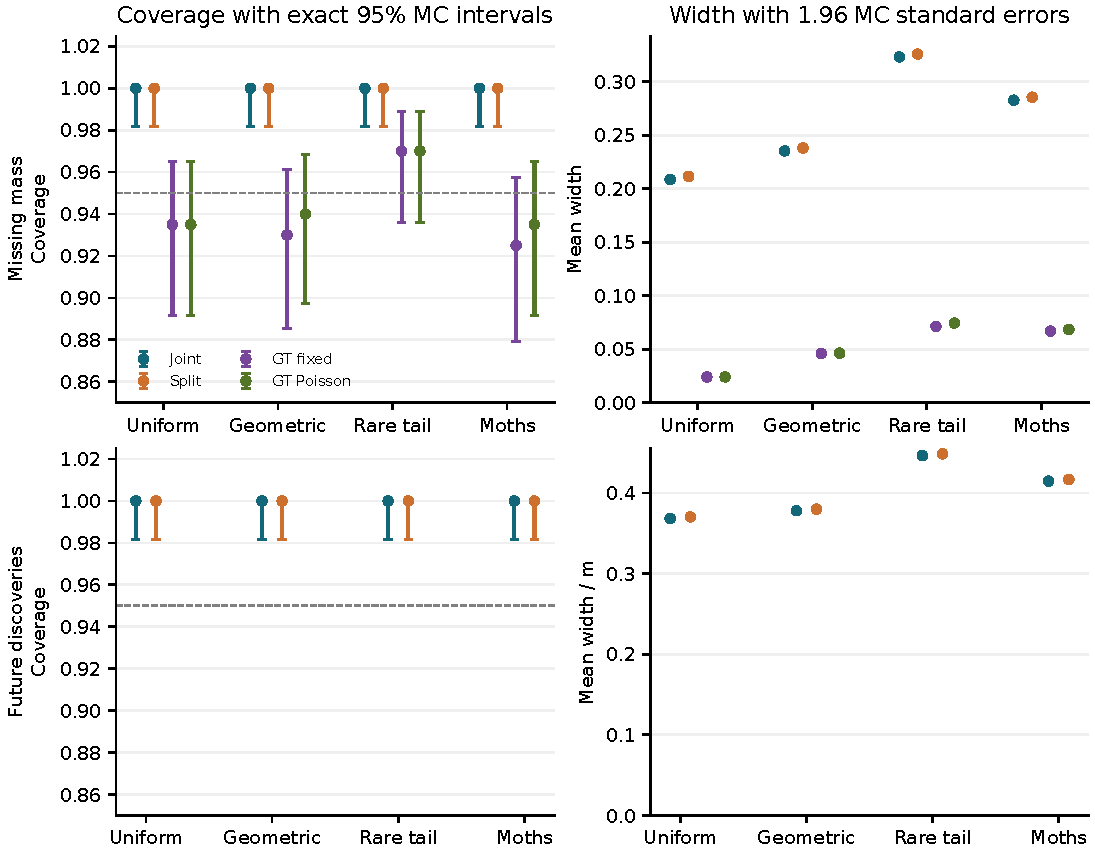
\includegraphics[width=\textwidth]{manuscripts/generated/coverage_width.pdf}
\caption{Paired results at $n=m=500$. Widths for discoveries are divided by
$m$ for display. The support benchmark, omitted from the plot, has coverage
one and normalized width one. Joint and split points often nearly coincide.
Intervals show Monte Carlo uncertainty, not confidence sets for population
parameters.}\label{fig:comparison}
\end{figure}

\subsection{Observed performance and computational accounting}
In all eight scenarios, both certified methods covered every simulated target.
With only 200 replicates, 200 successes still have a two-sided exact Monte Carlo
lower limit about 0.982. Thus the results are compatible with substantial
conservatism; they are not evidence that coverage equals one in general.
At $n=500$, joint missing-mass mean widths range from about 0.209 to 0.323,
whereas normal Good--Turing widths range from 0.024 to 0.071. The normal
method's corresponding coverage fractions are 0.935, 0.930, 0.970, and 0.925
for the four listed populations. The Poisson-variance variant gives
0.935, 0.940, 0.970, and 0.935, with slightly larger mean widths.
Those differences are reported with their
Monte Carlo uncertainty in the appendix.

The improvement over split calibration is modest: about 0.0027--0.0028 in
mean missing-mass width and one discovery in mean prediction width at
$n=500$. Both methods remain far narrower than full support but much wider
than one would want for precise prediction. These results motivate better
fixed directions, effort optimization, stronger nuisance constraints, and
more efficient continuum support bounds. They do not demonstrate that the
joint approach is competitive with all existing specialized procedures.

The study saves 1,438 distinct simulated fingerprints/designs and their
certificates, avoiding repeated optimization for identical inputs. Of 2,876
simulation endpoint proposals, 2,858 have solver status optimal and a verified
primal witness; 18 use a certified single-direction fallback. The fallback
cases remain in every coverage and width summary. Twelve additional
certificates cover the classical abundance examples. Shared kernel tables,
case-level intervals, truths, and the random seed are committed with the code.

\section{Serial numbers and the historical-data boundary}
For a uniform sample of $k$ distinct serials from $\{1,\ldots,N\}$ with maximum
$Z$, the classical German tank estimate is
$\widehat N=(k+1)Z/k-1$, and
\[
 \PP_N(Z\le z)=\binom zk\big/\binom Nk.
\]
The discovery companion develops exact inversion and a finite decision game.
This is a separate experiment: a serial's numerical value is informative,
whereas arbitrary species names or animal tags generally are not. A fleet
count inferred from repeated taxi sightings is therefore not automatically
a German tank analysis of the same observations.

\Cref{tab:wartime} preserves the published aggregate comparison as reproduced
by Miller, Sharma and Yang \cite[Fig.~1]{Miller2024}, who attribute it to
Ruggles and Brodie \cite{Ruggles1947}. Statistical estimates have smaller
absolute errors than the intelligence estimates in these three displayed
cases. This is a descriptive comparison of reported estimates with later
records, not a repeated-sampling coverage experiment. The table does not
identify the raw samples or establish that each historical estimate was
computed by the single-maximum formula above.

\begin{table}[htbp]\centering\small
\caption{Historical aggregate comparison from a documented secondary
reproduction. The final column is the statistical estimate's signed percent
error relative to the recorded total. No new serial-sample inference is implied.}
\label{tab:wartime}
\begin{tabular}{lrrrr}\toprule
Month & Intelligence & Statistical & Records & Error (\%)\\\midrule
\tableinput{manuscripts/generated/wartime.tex}
\bottomrule\end{tabular}
\end{table}

The Yale finding aid identifies Richard Ruggles Papers,
MS 1871, box 1, folder 2 for the 1947 article and folders 4--6 for tank and
tire production reports from 1943--1944 \cite{Yale}. This audit did not recover
an authenticated raw serial-number sample with a documented selection rule.
Consequently, no new raw-serial point estimate or confidence interval is
computed here. Aggregate production comparisons and archival locators are not
substitutes for raw observations. If the wartime summary is the only observed
statistic, its known coarsening map can be composed with a specified serial
sampling kernel and calibrated directly. Without that map and selection rule,
the admissible records or observation laws must remain nuisance variables;
an identified set may then be broad. This is a limitation of supplied
information, not an exclusion of aggregate data from the methodology.
Existing synthetic finite-game checks remain
labeled as such. Historical serial inference is a documented data-availability
limit of this draft, not a completed empirical case.

\section{Relation to established estimators and remaining work}
Good--Turing supplies the singleton-based missing-mass score
\cite{Good1953}; Good--Toulmin supplies alternating discovery coordinates
\cite{GoodToulmin1956}. Efron--Thisted's vocabulary application and linear
programming perspective are direct predecessors \cite{EfronThisted1976}.
Chao-type moment inequalities motivate the richness summaries
\cite{Chao1984,Chao1987}. None of these classical identities is new here.
The computational contribution is a replayable continuum enclosure for a
specified joint region, with numerical and statistical uncertainty separated.

Lincoln--Petersen and Chapman are evaluated under the two-sample
without-replacement model. Bailey's correction belongs to a different
with-replacement second sample; applying it indiscriminately to these records
would change the experiment. Schnabel and Schumacher--Eschmeyer use ordered
recapture information. Horvitz--Thompson requires specified inclusion
probabilities, which these historical frequency tables do not supply.
Inverse-sampling estimators require a stopping rule based on a prescribed
recapture count, not a fixed number of field occasions. Their exact recovery,
bias and calibration results remain in the capture--recapture companion
\cite{LongCapture}; listing them does not assert that every historical dataset
supports every estimator.

Smoothed Good--Toulmin and other modern unseen-species predictors deserve a
separate matched prediction study under their stated loss and horizon regimes.
This first interval benchmark does not establish superiority over those
methods, over specialized concentration intervals, or over heterogeneity-aware
capture models. Finite upper confidence bounds on total richness also need
additional restrictions; the mass and fixed-horizon guarantees do not by
themselves supply them. Before any priority or optimality claim, theorem-level
comparisons with the relevant literature are needed.

\section{Reproduction and recovery provenance}
The implementation and source data are in
\href{https://github.com/long-mathematics/partial-population-inference}{the project repository}.
Python 3.12 with the pinned empirical requirements supplies NumPy, SciPy,
CVXPY 1.9.3, CLARABEL 0.11.1, and python-flint 0.9.0. Exact versions are
recorded in \texttt{requirements-empirical.txt}. Standard TeX tools build the
paper; its tables and figure are generated from the checked JSON results.

\begin{samepage}\begin{verbatim}
python -m pip install -r requirements-empirical.txt
make check
make pdf
\end{verbatim}\end{samepage}
To regenerate data transformations and simulations, rather than replay saved
certificates, run the extraction, classical analysis, coverage study, and
table-generation scripts described in the verification guide. The projection
command accepts the known $n$, the required fingerprint coordinates, and a
prespecified future size; its separate verification mode does not call the
optimizer. The finite-law test suite enumerates small rational multinomial
experiments, checks e-value expectations, rejects forged tables and endpoints,
and forces solver failure. General validity rests on the displayed proof,
not on a finite list of test populations.

This version reconstructs the unfinished implementation from the published
theory and preserved source records after the earlier Work-context recovery
archive could not be downloaded. It does not claim byte-for-byte recovery of
that unpublished implementation or reproduce its reported certificate count.
The baseline four theory manuscripts are retained; this paper, its implementation,
data manifest, and replay artifacts form a separately auditable addition.

\clearpage\appendix
\section{Complete paired simulation summaries}
The final column gives mean width with Monte Carlo standard error in
parentheses. Brackets in the coverage column are exact binomial Monte Carlo
95\% intervals. Width is in probability units for mass and integer-count
units for discoveries. All rows use 200 replicates.

\small
\begin{longtable}{rllrr}
\caption{Realized missing mass.}\label{tab:allmass}\\
\toprule $n$ & Population & Method & Coverage [MC interval] & Mean width (SE)\\\midrule
\endfirsthead
\toprule $n$ & Population & Method & Coverage [MC interval] & Mean width (SE)\\\midrule
\endhead
\bottomrule\endfoot
\tableinput{manuscripts/generated/simulation_missing_mass.tex}
\end{longtable}
\begin{longtable}{rllrr}
\caption{Realized future discoveries, $m=n$.}\label{tab:allfuture}\\
\toprule $n$ & Population & Method & Coverage [MC interval] & Mean width (SE)\\\midrule
\endfirsthead
\toprule $n$ & Population & Method & Coverage [MC interval] & Mean width (SE)\\\midrule
\endhead
\bottomrule\endfoot
\tableinput{manuscripts/generated/simulation_discoveries.tex}
\end{longtable}
\normalsize

\clearpage
\begin{thebibliography}{99}\small\raggedright
\bibitem{Anan2017} O. Anan, D. B\"ohning, and A. Maruotti. Uncertainty
estimation in heterogeneous capture--recapture count data.
\emph{Journal of Statistical Computation and Simulation} 87 (2017), 2094--2114.
\href{https://doi.org/10.1080/00949655.2017.1315668}{doi:10.1080/00949655.2017.1315668}.
\bibitem{Chen} C. Yu. \emph{The Use of Mixture Models in Capture--Recapture}.
PhD thesis, University of Kent (2015), Table 2.1, p.~13.
\url{https://kar.kent.ac.uk/50775/1/218Chen_Yu.pdf}.
\bibitem{Krebs} C. J. Krebs. Estimating abundance and density: Mark-recapture
techniques, chapter 2, Table 2.2, p.~46, online teaching chapter.
\url{https://www.zoology.ubc.ca/~krebs/downloads/krebs_chapter_02_2021.pdf}.
\bibitem{Ridout} M. S. Ridout. Software for fitting capture heterogeneity
models to estimate the size of a closed population, version 1.0 (2007), p.~2.
\url{https://www.kent.ac.uk/smsas/personal/msr/webfiles/estimateN/estimateN.pdf}.
\bibitem{Baillargeon2007} S. Baillargeon and L.-P. Rivest.
Rcapture: Loglinear models for capture--recapture in R.
\emph{Journal of Statistical Software} 19(5) (2007).
\href{https://doi.org/10.18637/jss.v019.i05}{doi:10.18637/jss.v019.i05}.
\bibitem{Carothers1973} A. D. Carothers. The effects of unequal catchability on
Jolly--Seber estimates. \emph{Journal of Animal Ecology} 42 (1973), 125--146.
\bibitem{Chao1984} A. Chao. Nonparametric estimation of the number of classes
in a population. \emph{Scandinavian Journal of Statistics} 11 (1984), 265--270.
\bibitem{Chao1987} A. Chao. Estimating the population size for capture--recapture
data with unequal catchability. \emph{Biometrics} 43 (1987), 783--791.
\bibitem{Condit2002} R. Condit et al. Beta-diversity in tropical forest trees.
\emph{Science} 295 (2002), 666--669.
\href{https://doi.org/10.1126/science.1066854}{doi:10.1126/science.1066854}.
\bibitem{Edwards1967} W. R. Edwards and L. L. Eberhardt. Estimating cottontail
abundance from live trapping data. \emph{Journal of Wildlife Management} 31
(1967), 87--96.
\bibitem{EfronThisted1976} B. Efron and R. Thisted. Estimating the number of
unseen species: How many words did Shakespeare know? \emph{Biometrika} 63
(1976), 435--447.
\bibitem{Esty1983} W. W. Esty. A normal limit law for a nonparametric estimator
of the coverage of a random sample. \emph{Annals of Statistics} 11 (1983), 905--912.
\bibitem{Fisher1943} R. A. Fisher, A. S. Corbet, and C. B. Williams. The relation
between the number of species and the number of individuals in a random sample
of an animal population. \emph{Journal of Animal Ecology} 12 (1943), 42--58.
\bibitem{Good1953} I. J. Good. The population frequencies of species and the
estimation of population parameters. \emph{Biometrika} 40 (1953), 237--264.
\bibitem{GoodToulmin1956} I. J. Good and G. H. Toulmin. The number of new species,
and the increase in population coverage, when a sample is increased.
\emph{Biometrika} 43 (1956), 45--63.
\bibitem{Johansson2017} F. Johansson. Arb: Efficient arbitrary-precision
midpoint-radius interval arithmetic. \emph{IEEE Transactions on Computers}
66 (2017), 1281--1292. \href{https://doi.org/10.1109/TC.2017.2690633}{doi:10.1109/TC.2017.2690633}.
\bibitem{PythonFlint} python-flint developers. Real ball arithmetic
(\texttt{arb}), documentation for python-flint.
\url{https://python-flint.readthedocs.io/en/stable/arb.html}. Accessed November 17, 2026.
\bibitem{CVXPY} S. Diamond and S. Boyd. CVXPY: A Python-embedded modeling
language for convex optimization. \emph{Journal of Machine Learning Research}
17(83) (2016), 1--5. \url{https://www.jmlr.org/papers/v17/15-408.html}.
\bibitem{Clarabel} Clarabel developers. Clarabel documentation, exponential-cone
solver. \url{https://clarabel.org/stable/}. Accessed November 17, 2026.
\bibitem{LongDiscovery} C. D. Long. Discovery-rate inversion. Companion
research draft, version 0.2 (2026), project repository.
\bibitem{LongTransfer} C. D. Long. Transfer and generation. Companion
research draft (2026), project repository.
\bibitem{LongCumulants} C. D. Long. Additive cumulants and fixed-sample
computation. Companion research draft (2026), project repository.
\bibitem{LongCapture} C. D. Long. Capture--recapture in a sampling-kernel
framework. Companion research draft, version 0.1 (2026), project repository.
\bibitem{McCrea2014} R. S. McCrea and B. J. T. Morgan. \emph{Analysis of
Capture--Recapture Data}. Chapman \& Hall/CRC, 2014. Table 3.1 companion workbook,
\url{https://www.capturerecapture.co.uk/datasets.html}.
\bibitem{Preston1948} F. W. Preston. The commonness, and rarity, of species.
\emph{Ecology} 29 (1948), 254--283.
\bibitem{Ricker1975} W. E. Ricker. \emph{Computation and Interpretation of
Biological Statistics of Fish Populations}. Bulletin 191, Fisheries Research
Board of Canada, 1975. Dahl example as documented in \texttt{Petersen}.
\bibitem{Miller2024} S. J. Miller, K. Sharma, and A. K. Yang.
The German tank problem with multiple factories. \emph{The PUMP Journal of
Undergraduate Research} 7 (2024), 231--257.
\url{https://par.nsf.gov/servlets/purl/10580624}.
\bibitem{Ruggles1947} R. Ruggles and H. Brodie. An empirical approach to economic
intelligence in World War II. \emph{Journal of the American Statistical
Association} 42 (1947), 72--91.
\href{https://doi.org/10.1080/01621459.1947.10501915}{doi:10.1080/01621459.1947.10501915}.
\bibitem{Yale} Yale University Library. \emph{Guide to the Richard Ruggles
Papers}, MS 1871, compiled by Scott Libson (2006), finding aid exported 2025.
\url{https://hdl.handle.net/10079/fa/mssa.ms.1871}.
\bibitem{ZhangZhang2009} C.-H. Zhang and Z. Zhang. Asymptotic normality of a
nonparametric estimator of sample coverage. \emph{Annals of Statistics} 37
(2009), 2582--2595. \href{https://doi.org/10.1214/08-AOS658}{doi:10.1214/08-AOS658}.
\end{thebibliography}
\end{document}
